\section{Bandits of Eagle Mountain}

Over dinner with Mia, the party learns that they have been assembled to try and restore faith in law and order in Losokyo. Mia gives a brief history of the rise and fall of the Losokyan legal system. If pressed, she can also describe \linkto{events:dl6} and \linkto{events:kidnapdh}.
Talking with people around town about the bandit problem, the party learns that the city has almost been under seige for the last year because of bandits. Trade caravans need to have substantial escorts, as the bandits always seem to know when conveys are scheduled to leave or arrive\footnote{Redd White's Bluecorp is behind this}. Losokyan militias have scoured the countryside looking for the bandit camp, but have not found any trace of one.

One particularly intrepid journalist, \linkto{people:lotta}, has been investigating rumors of a ``Pasquash'' in the forested mountains east of the city. In that process, she stumbled across wagon tracks leading to the edge of the ravine of Eagle River, in the Eagle Mountains. 

\subsection{Eagle Mountain}
High up in the mountains, the road leads to a cliff with a wooden bridge spanning the chasm to the other side. Smaller paths head further up the mountain on this side of the chasm. At the bottom of the chasm, 50 feet below, the Eagle River rages, although the area under the bridge on the far side is a rocky bank, about 10 feet above the river. 

To the south, a large cliff prevents vision beyond about 30 feet, although brilliant colored shapes can be seen occasionally peeking above the ridge. On the near-side cliff wall, about 20 feet down, there is a cave. 

\subsection{The Cave}
The cave quickly opens up into a large room, with a dozen statues lining the left and right walls and one placed near the middle of the room, apparently figures in the middle of various actions, mostly seeming to be in combat. Each statue has a couple glyphs written on its base. The statue in the center is a statue of King Primidux, facing to the right with his hands, and sword, facing the left. On the opposite wall, a message, encoded in glyphs, is engraved in marble that has been carefully inserted into the stone wall. To either side of the message, magical flames give the room a dim light. Along the sides of the room, a sequence of 30 glyphs occur on either side, both in the same order\footnote{It's the alphabet and ,.!?}. In the center of the room, there are 25 depressions in the ground that match the shape of the bases of the statues. In the center of that circle, there is a smooth orb.

\subsection{The Puzzle}
To proceed, the statues must be placed in their correct locations in the circle. When in the correct location, the glyphs on the statues when read counterclockwise starting with King Primidux replicate the message engraved on the front wall. A high intelligence roll or smart player might realize the glyphs on the walls are meant to be an alphabet, which allows them to decode the message:
\begin{center}

\includegraphics[scale=0.5]{combats/alphabet.PNG}\\
- The ``Alphabet''\\

``abcdefghijklmnopqrstuvwxyz,.!?''\\
- The alphabet, decoded\\

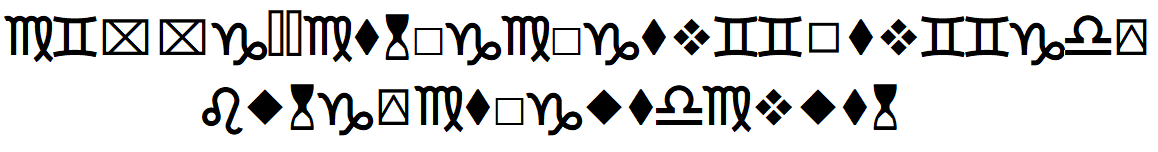
\includegraphics[scale=0.5]{combats/message.PNG}\\
- The message, divided into the statues \\

``Those who inherit our will shall shine in the middle''\\
- The message, decoded
\end{center}

The message is actually backwards, and so reading \textit{clockwise} reveals the meaning of the message. When the statues are placed in the right order, a door underneath the engraving opens, however this door is alarmed. The alarm will be disabled if a bright light is shone upon the orb in the center; when that happens, the orb will emit its own bright, pale green, light.

\subsection{The Bandit Hideout}
The bandits' initial positions are as follows:
\begin{itemize}
\item Four are asleep in the quarters
\item One is patrolling the main hallway
\item Three are meeting in the office
\item Stella Artois is in her study
\end{itemize}
If the alarm is tripped, all the bandits will move to the Great Hall to ambush the party when they walk in, except one, which will be in the watchroom.